% Source: graduate-coursework/Prior_Semesters/Fa23/ELCT432/exercises/PA4_FM_Carsons_Rule.tex

\documentclass[border=4pt]{standalone}
\usepackage{amsmath,amsfonts,amssymb}
\usepackage{graphicx}
\usepackage{tikz}
\usetikzlibrary{arrows}

\begin{document}
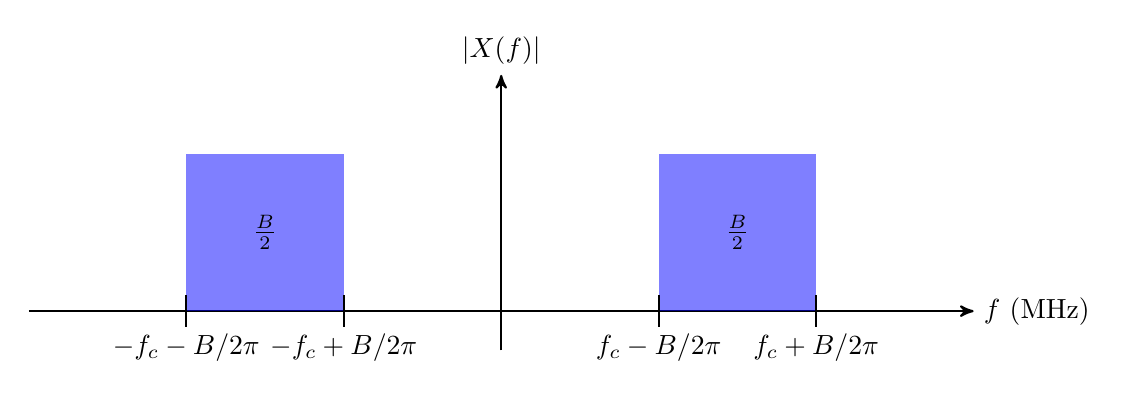
\begin{tikzpicture}[>=stealth']
    % Draw x-axis and y-axis
    \draw[thick,->] (-6,0) -- (6,0) node[right] { \( f \) (MHz)};
    \draw[thick,->] (0,-0.5) -- (0,3) node[above] { \( |X(f)| \) };

    % Draw rectangles for frequency components
    \fill[blue,opacity=0.5] (-4,0) rectangle (-2,2);
    \fill[blue,opacity=0.5] (2,0) rectangle (4,2);

    % Label frequency components
    \node at (-3,1) { \( \frac{B}{2} \) };
    \node at (3,1) { \( \frac{B}{2} \) };

    % Label frequency values
    \draw[thick] (-2,-0.2) -- (-2,0.2) node[below=10pt] { \( -f_c + B/2\pi \) };
    \draw[thick] (-4,-0.2) -- (-4,0.2) node[below=10pt] { \( -f_c - B/2\pi \) };
    \draw[thick] (2,-0.2) -- (2,0.2) node[below=10pt] { \( f_c - B/2\pi \) };
    \draw[thick] (4,-0.2) -- (4,0.2) node[below=10pt] { \( f_c + B/2\pi \) };
\end{tikzpicture}
\end{document}
